% Options for packages loaded elsewhere
\PassOptionsToPackage{unicode}{hyperref}
\PassOptionsToPackage{hyphens}{url}
\PassOptionsToPackage{dvipsnames,svgnames,x11names}{xcolor}
%
\documentclass[
  letterpaper,
  DIV=11,
  numbers=noendperiod]{scrartcl}

\usepackage{amsmath,amssymb}
\usepackage{iftex}
\ifPDFTeX
  \usepackage[T1]{fontenc}
  \usepackage[utf8]{inputenc}
  \usepackage{textcomp} % provide euro and other symbols
\else % if luatex or xetex
  \usepackage{unicode-math}
  \defaultfontfeatures{Scale=MatchLowercase}
  \defaultfontfeatures[\rmfamily]{Ligatures=TeX,Scale=1}
\fi
\usepackage{lmodern}
\ifPDFTeX\else  
    % xetex/luatex font selection
\fi
% Use upquote if available, for straight quotes in verbatim environments
\IfFileExists{upquote.sty}{\usepackage{upquote}}{}
\IfFileExists{microtype.sty}{% use microtype if available
  \usepackage[]{microtype}
  \UseMicrotypeSet[protrusion]{basicmath} % disable protrusion for tt fonts
}{}
\makeatletter
\@ifundefined{KOMAClassName}{% if non-KOMA class
  \IfFileExists{parskip.sty}{%
    \usepackage{parskip}
  }{% else
    \setlength{\parindent}{0pt}
    \setlength{\parskip}{6pt plus 2pt minus 1pt}}
}{% if KOMA class
  \KOMAoptions{parskip=half}}
\makeatother
\usepackage{xcolor}
\setlength{\emergencystretch}{3em} % prevent overfull lines
\setcounter{secnumdepth}{-\maxdimen} % remove section numbering
% Make \paragraph and \subparagraph free-standing
\makeatletter
\ifx\paragraph\undefined\else
  \let\oldparagraph\paragraph
  \renewcommand{\paragraph}{
    \@ifstar
      \xxxParagraphStar
      \xxxParagraphNoStar
  }
  \newcommand{\xxxParagraphStar}[1]{\oldparagraph*{#1}\mbox{}}
  \newcommand{\xxxParagraphNoStar}[1]{\oldparagraph{#1}\mbox{}}
\fi
\ifx\subparagraph\undefined\else
  \let\oldsubparagraph\subparagraph
  \renewcommand{\subparagraph}{
    \@ifstar
      \xxxSubParagraphStar
      \xxxSubParagraphNoStar
  }
  \newcommand{\xxxSubParagraphStar}[1]{\oldsubparagraph*{#1}\mbox{}}
  \newcommand{\xxxSubParagraphNoStar}[1]{\oldsubparagraph{#1}\mbox{}}
\fi
\makeatother

\usepackage{color}
\usepackage{fancyvrb}
\newcommand{\VerbBar}{|}
\newcommand{\VERB}{\Verb[commandchars=\\\{\}]}
\DefineVerbatimEnvironment{Highlighting}{Verbatim}{commandchars=\\\{\}}
% Add ',fontsize=\small' for more characters per line
\usepackage{framed}
\definecolor{shadecolor}{RGB}{241,243,245}
\newenvironment{Shaded}{\begin{snugshade}}{\end{snugshade}}
\newcommand{\AlertTok}[1]{\textcolor[rgb]{0.68,0.00,0.00}{#1}}
\newcommand{\AnnotationTok}[1]{\textcolor[rgb]{0.37,0.37,0.37}{#1}}
\newcommand{\AttributeTok}[1]{\textcolor[rgb]{0.40,0.45,0.13}{#1}}
\newcommand{\BaseNTok}[1]{\textcolor[rgb]{0.68,0.00,0.00}{#1}}
\newcommand{\BuiltInTok}[1]{\textcolor[rgb]{0.00,0.23,0.31}{#1}}
\newcommand{\CharTok}[1]{\textcolor[rgb]{0.13,0.47,0.30}{#1}}
\newcommand{\CommentTok}[1]{\textcolor[rgb]{0.37,0.37,0.37}{#1}}
\newcommand{\CommentVarTok}[1]{\textcolor[rgb]{0.37,0.37,0.37}{\textit{#1}}}
\newcommand{\ConstantTok}[1]{\textcolor[rgb]{0.56,0.35,0.01}{#1}}
\newcommand{\ControlFlowTok}[1]{\textcolor[rgb]{0.00,0.23,0.31}{\textbf{#1}}}
\newcommand{\DataTypeTok}[1]{\textcolor[rgb]{0.68,0.00,0.00}{#1}}
\newcommand{\DecValTok}[1]{\textcolor[rgb]{0.68,0.00,0.00}{#1}}
\newcommand{\DocumentationTok}[1]{\textcolor[rgb]{0.37,0.37,0.37}{\textit{#1}}}
\newcommand{\ErrorTok}[1]{\textcolor[rgb]{0.68,0.00,0.00}{#1}}
\newcommand{\ExtensionTok}[1]{\textcolor[rgb]{0.00,0.23,0.31}{#1}}
\newcommand{\FloatTok}[1]{\textcolor[rgb]{0.68,0.00,0.00}{#1}}
\newcommand{\FunctionTok}[1]{\textcolor[rgb]{0.28,0.35,0.67}{#1}}
\newcommand{\ImportTok}[1]{\textcolor[rgb]{0.00,0.46,0.62}{#1}}
\newcommand{\InformationTok}[1]{\textcolor[rgb]{0.37,0.37,0.37}{#1}}
\newcommand{\KeywordTok}[1]{\textcolor[rgb]{0.00,0.23,0.31}{\textbf{#1}}}
\newcommand{\NormalTok}[1]{\textcolor[rgb]{0.00,0.23,0.31}{#1}}
\newcommand{\OperatorTok}[1]{\textcolor[rgb]{0.37,0.37,0.37}{#1}}
\newcommand{\OtherTok}[1]{\textcolor[rgb]{0.00,0.23,0.31}{#1}}
\newcommand{\PreprocessorTok}[1]{\textcolor[rgb]{0.68,0.00,0.00}{#1}}
\newcommand{\RegionMarkerTok}[1]{\textcolor[rgb]{0.00,0.23,0.31}{#1}}
\newcommand{\SpecialCharTok}[1]{\textcolor[rgb]{0.37,0.37,0.37}{#1}}
\newcommand{\SpecialStringTok}[1]{\textcolor[rgb]{0.13,0.47,0.30}{#1}}
\newcommand{\StringTok}[1]{\textcolor[rgb]{0.13,0.47,0.30}{#1}}
\newcommand{\VariableTok}[1]{\textcolor[rgb]{0.07,0.07,0.07}{#1}}
\newcommand{\VerbatimStringTok}[1]{\textcolor[rgb]{0.13,0.47,0.30}{#1}}
\newcommand{\WarningTok}[1]{\textcolor[rgb]{0.37,0.37,0.37}{\textit{#1}}}

\providecommand{\tightlist}{%
  \setlength{\itemsep}{0pt}\setlength{\parskip}{0pt}}\usepackage{longtable,booktabs,array}
\usepackage{calc} % for calculating minipage widths
% Correct order of tables after \paragraph or \subparagraph
\usepackage{etoolbox}
\makeatletter
\patchcmd\longtable{\par}{\if@noskipsec\mbox{}\fi\par}{}{}
\makeatother
% Allow footnotes in longtable head/foot
\IfFileExists{footnotehyper.sty}{\usepackage{footnotehyper}}{\usepackage{footnote}}
\makesavenoteenv{longtable}
\usepackage{graphicx}
\makeatletter
\def\maxwidth{\ifdim\Gin@nat@width>\linewidth\linewidth\else\Gin@nat@width\fi}
\def\maxheight{\ifdim\Gin@nat@height>\textheight\textheight\else\Gin@nat@height\fi}
\makeatother
% Scale images if necessary, so that they will not overflow the page
% margins by default, and it is still possible to overwrite the defaults
% using explicit options in \includegraphics[width, height, ...]{}
\setkeys{Gin}{width=\maxwidth,height=\maxheight,keepaspectratio}
% Set default figure placement to htbp
\makeatletter
\def\fps@figure{htbp}
\makeatother

\KOMAoption{captions}{tableheading}
\makeatletter
\@ifpackageloaded{caption}{}{\usepackage{caption}}
\AtBeginDocument{%
\ifdefined\contentsname
  \renewcommand*\contentsname{Table of contents}
\else
  \newcommand\contentsname{Table of contents}
\fi
\ifdefined\listfigurename
  \renewcommand*\listfigurename{List of Figures}
\else
  \newcommand\listfigurename{List of Figures}
\fi
\ifdefined\listtablename
  \renewcommand*\listtablename{List of Tables}
\else
  \newcommand\listtablename{List of Tables}
\fi
\ifdefined\figurename
  \renewcommand*\figurename{Figure}
\else
  \newcommand\figurename{Figure}
\fi
\ifdefined\tablename
  \renewcommand*\tablename{Table}
\else
  \newcommand\tablename{Table}
\fi
}
\@ifpackageloaded{float}{}{\usepackage{float}}
\floatstyle{ruled}
\@ifundefined{c@chapter}{\newfloat{codelisting}{h}{lop}}{\newfloat{codelisting}{h}{lop}[chapter]}
\floatname{codelisting}{Listing}
\newcommand*\listoflistings{\listof{codelisting}{List of Listings}}
\makeatother
\makeatletter
\makeatother
\makeatletter
\@ifpackageloaded{caption}{}{\usepackage{caption}}
\@ifpackageloaded{subcaption}{}{\usepackage{subcaption}}
\makeatother

\ifLuaTeX
  \usepackage{selnolig}  % disable illegal ligatures
\fi
\usepackage{bookmark}

\IfFileExists{xurl.sty}{\usepackage{xurl}}{} % add URL line breaks if available
\urlstyle{same} % disable monospaced font for URLs
\hypersetup{
  pdftitle={Problem Set 2 Answer},
  colorlinks=true,
  linkcolor={blue},
  filecolor={Maroon},
  citecolor={Blue},
  urlcolor={Blue},
  pdfcreator={LaTeX via pandoc}}


\title{Problem Set 2 Answer}
\author{}
\date{}

\begin{document}
\maketitle


\begin{enumerate}
\def\labelenumi{\arabic{enumi}.}
\tightlist
\item
  ``This submission is my work alone and complies with the 30538
  integrity policy.'' Add your initials to indicate your agreement:
  \textbf{\emph{HX}}
\item
  ``I have uploaded the names of anyone I worked with on the problem set
  here'' \textbf{\emph{HX}} (2 point)
\item
  Late coins used this pset: \textbf{\emph{0}} Late coins left after
  submission: \textbf{\emph{4}} 4. Knit your ps2.qmd to a pdf named
  ps2.pdf. • The PDF should not be more than 25 pages. Use head() and
  re-size figures when appropriate.
\item
  Push ps2.qmd and ps2.pdf to your github repo. It is fine to use Github
  Desktop. 6. Submit ps2.pdf via Gradescope (8 points)
\item
  Tag your submission in Gradescope
\end{enumerate}

\begin{Shaded}
\begin{Highlighting}[]
\ImportTok{import}\NormalTok{ pandas }\ImportTok{as}\NormalTok{ pd}
\ImportTok{import}\NormalTok{ altair }\ImportTok{as}\NormalTok{ alt}
\ImportTok{import}\NormalTok{ os}
\NormalTok{alt.renderers.enable(}\StringTok{\textquotesingle{}png\textquotesingle{}}\NormalTok{)}

\CommentTok{\# Read in the csv file}
\CommentTok{\# Warning message is suppressed for output clarity.}
\NormalTok{data }\OperatorTok{=}\NormalTok{ pd.read\_csv(}
    \StringTok{\textquotesingle{}problem\_sets/ps2/data/parking\_tickets\_one\_percent.csv\textquotesingle{}}\NormalTok{, }
\NormalTok{    index\_col}\OperatorTok{=}\NormalTok{[}\DecValTok{0}\NormalTok{]}
\NormalTok{    )}
\NormalTok{df }\OperatorTok{=}\NormalTok{ pd.DataFrame(data)}
\end{Highlighting}
\end{Shaded}

\subsection{Data Cleaning continued}\label{data-cleaning-continued}

\textbf{\emph{Q1}}

\begin{Shaded}
\begin{Highlighting}[]
\CommentTok{\# Define the function to count NAs}
\KeywordTok{def}\NormalTok{ count\_na(df):}
\NormalTok{    labels }\OperatorTok{=}\NormalTok{ []  }
\NormalTok{    na\_counts }\OperatorTok{=}\NormalTok{ [] }
    \ControlFlowTok{for}\NormalTok{ label, content }\KeywordTok{in}\NormalTok{ df.items():}
\NormalTok{        count }\OperatorTok{=}\NormalTok{ content.isna().}\BuiltInTok{sum}\NormalTok{()}
\NormalTok{        labels.append(label)}
\NormalTok{        na\_counts.append(count)}
\NormalTok{    result\_dict }\OperatorTok{=}\NormalTok{ \{}\StringTok{\textquotesingle{}Variable\textquotesingle{}}\NormalTok{: labels, }\StringTok{\textquotesingle{}NA Count\textquotesingle{}}\NormalTok{: na\_counts\}}
\NormalTok{    result\_df }\OperatorTok{=}\NormalTok{ pd.DataFrame.from\_dict(result\_dict)}
    \ControlFlowTok{return}\NormalTok{ result\_df}


\CommentTok{\# Conduct a test}
\NormalTok{df\_test }\OperatorTok{=}\NormalTok{ pd.DataFrame(\{}
    \StringTok{\textquotesingle{}A\textquotesingle{}}\NormalTok{: [}\DecValTok{1}\NormalTok{, }\DecValTok{2}\NormalTok{, }\VariableTok{None}\NormalTok{, }\VariableTok{None}\NormalTok{],}
    \StringTok{\textquotesingle{}B\textquotesingle{}}\NormalTok{: [}\DecValTok{1}\NormalTok{, }\DecValTok{2}\NormalTok{, }\DecValTok{3}\NormalTok{, }\DecValTok{4}\NormalTok{],}
    \StringTok{\textquotesingle{}C\textquotesingle{}}\NormalTok{: [}\DecValTok{1}\NormalTok{, }\StringTok{\textquotesingle{}Apple\textquotesingle{}}\NormalTok{, }\DecValTok{3}\NormalTok{, }\VariableTok{None}\NormalTok{]}
\NormalTok{\})}
\BuiltInTok{print}\NormalTok{(df\_test, }\StringTok{\textquotesingle{}}\CharTok{\textbackslash{}n}\StringTok{\textquotesingle{}}\NormalTok{)}
\BuiltInTok{print}\NormalTok{(count\_na(df\_test), }\StringTok{\textquotesingle{}}\CharTok{\textbackslash{}n}\StringTok{\textquotesingle{}}\NormalTok{)}

\BuiltInTok{print}\NormalTok{(}\StringTok{\textquotesingle{}So the function works.}\CharTok{\textbackslash{}n}\StringTok{Applying to our dataset:\textquotesingle{}}\NormalTok{, }\StringTok{\textquotesingle{}}\CharTok{\textbackslash{}n}\StringTok{\textquotesingle{}}\NormalTok{)}
\BuiltInTok{print}\NormalTok{(count\_na(df))}
\end{Highlighting}
\end{Shaded}

\begin{verbatim}
     A  B      C
0  1.0  1      1
1  2.0  2  Apple
2  NaN  3      3
3  NaN  4   None 

  Variable  NA Count
0        A         2
1        B         0
2        C         1 

So the function works.
Applying to our dataset: 

                 Variable  NA Count
0           ticket_number         0
1              issue_date         0
2      violation_location         0
3    license_plate_number         0
4     license_plate_state        97
5      license_plate_type      2054
6                 zipcode     54115
7          violation_code         0
8   violation_description         0
9                    unit        29
10       unit_description         0
11           vehicle_make         0
12     fine_level1_amount         0
13     fine_level2_amount         0
14     current_amount_due         0
15         total_payments         0
16           ticket_queue         0
17      ticket_queue_date         0
18           notice_level     84068
19    hearing_disposition    259899
20          notice_number         0
21                officer         0
22                address         0
\end{verbatim}

\textbf{\emph{Q2}}

The zipcode, notice\_level and hearing\_disposition are missing much
more frequently than others, probably because of the way data was
collected. According to the dictionary, zipcode is the ZIP code
associated with the vehicle registration. If the registration
information is unclear or incomplete, this field might be left empty.
notice\_level describes the type of notice the city has sent a motorist.
If no notice was sent, this field would be blank. Similarly,
hearing\_disposition represents the outcome of a hearing. If the ticket
was not contested, this field would be blank.

In conclusion, these three variables contain more NAs than average
because of their data entry styles. These fields are filled only if
certain conditions are met, such as ticket got contested. Other
variables that capture essential information, such as ticket numbers and
issue dates, are routinely collected with each ticket issued. Thus, they
are more likely to be NA than others.

\textbf{\emph{Q3}}

\begin{Shaded}
\begin{Highlighting}[]
\NormalTok{df\_Q3 }\OperatorTok{=}\NormalTok{ df[df[}\StringTok{\textquotesingle{}violation\_description\textquotesingle{}}\NormalTok{].}\BuiltInTok{str}\NormalTok{.contains(}\StringTok{\textquotesingle{}NO CITY STICKER\textquotesingle{}}\NormalTok{, na}\OperatorTok{=}\VariableTok{False}\NormalTok{)]}
\BuiltInTok{print}\NormalTok{(df\_Q3[}\StringTok{\textquotesingle{}violation\_code\textquotesingle{}}\NormalTok{].unique()) }\CommentTok{\# Ordered by first apperance in dataset}
\end{Highlighting}
\end{Shaded}

\begin{verbatim}
['0964125' '0976170' '0964125B' '0964125C']
\end{verbatim}

By inspection, we know that 0976170 and 0964125C are extremely rare
cases in the dataset. Here we ignore these two values. Old violation
code: 0964125; New violation code: 0964125B. \newpage \textbf{\emph{Q4}}

Accoding to the articles, citations for not having a required vehicle
sticker rose from \$120 to \$200. So we have the cost under old
violation code: \$120; under new code: \$200. In the dataset, we refer
to the variable of fine\_level1\_amount.

\begin{Shaded}
\begin{Highlighting}[]
\CommentTok{\# For \textquotesingle{}0964125\textquotesingle{} }
\BuiltInTok{print}\NormalTok{(df[df[}\StringTok{\textquotesingle{}violation\_code\textquotesingle{}}\NormalTok{] }\OperatorTok{==} \StringTok{\textquotesingle{}0964125\textquotesingle{}}\NormalTok{][}\StringTok{\textquotesingle{}fine\_level1\_amount\textquotesingle{}}\NormalTok{].unique())}
\end{Highlighting}
\end{Shaded}

\begin{verbatim}
[120]
\end{verbatim}

\begin{Shaded}
\begin{Highlighting}[]
\CommentTok{\# For \textquotesingle{}0964125B\textquotesingle{} }
\BuiltInTok{print}\NormalTok{(df[df[}\StringTok{\textquotesingle{}violation\_code\textquotesingle{}}\NormalTok{] }\OperatorTok{==} \StringTok{\textquotesingle{}0964125B\textquotesingle{}}\NormalTok{][}\StringTok{\textquotesingle{}fine\_level1\_amount\textquotesingle{}}\NormalTok{].unique())}
\CommentTok{\# \textquotesingle{}0964125C\textquotesingle{} ignored as instructed.}
\end{Highlighting}
\end{Shaded}

\begin{verbatim}
[200]
\end{verbatim}

The result above aligns with the article. To be more specific, the cost
of an initial offense under 0964125 was \$120, and the cost of an
initial offense under 0964125B was \$200.

\subsection{Revenue increase from `missing city sticker'
tickets}\label{revenue-increase-from-missing-city-sticker-tickets}

\textbf{\emph{Q1}}

\begin{Shaded}
\begin{Highlighting}[]
\CommentTok{\# Unify the codes with 000}
\NormalTok{df\_unified }\OperatorTok{=}\NormalTok{ df.copy()}
\NormalTok{df\_unified }\OperatorTok{=}\NormalTok{  df\_unified.replace(}\StringTok{\textquotesingle{}0964125\textquotesingle{}}\NormalTok{, }\StringTok{\textquotesingle{}000\textquotesingle{}}\NormalTok{)}
\NormalTok{df\_unified }\OperatorTok{=}\NormalTok{  df\_unified.replace(}\StringTok{\textquotesingle{}0964125B\textquotesingle{}}\NormalTok{, }\StringTok{\textquotesingle{}000\textquotesingle{}}\NormalTok{)}
\NormalTok{df\_unified }\OperatorTok{=}\NormalTok{ df\_unified[df\_unified[}\StringTok{\textquotesingle{}violation\_code\textquotesingle{}}\NormalTok{] }\OperatorTok{==} \StringTok{\textquotesingle{}000\textquotesingle{}}\NormalTok{]}
\CommentTok{\# Extract year{-}month and count}
\NormalTok{df\_unified[}\StringTok{\textquotesingle{}issue\_date\textquotesingle{}}\NormalTok{] }\OperatorTok{=}\NormalTok{ pd.to\_datetime(}
\NormalTok{df\_unified[}\StringTok{\textquotesingle{}issue\_date\textquotesingle{}}\NormalTok{])}
\NormalTok{df\_unified[}\StringTok{\textquotesingle{}issue\_y\_m\textquotesingle{}}\NormalTok{] }\OperatorTok{=}\NormalTok{ df\_unified[}\StringTok{\textquotesingle{}issue\_date\textquotesingle{}}\NormalTok{].dt.strftime(}\StringTok{\textquotesingle{}\%Y{-}\%m\textquotesingle{}}\NormalTok{)}
\NormalTok{grouped\_date }\OperatorTok{=}\NormalTok{ df\_unified.groupby(}\StringTok{\textquotesingle{}issue\_y\_m\textquotesingle{}}\NormalTok{)}
\NormalTok{Q1\_count }\OperatorTok{=}\NormalTok{ grouped\_date.size().reset\_index(name}\OperatorTok{=}\StringTok{\textquotesingle{}count\textquotesingle{}}\NormalTok{)}
\BuiltInTok{print}\NormalTok{(Q1\_count.head(}\DecValTok{10}\NormalTok{))}

\CommentTok{\# Aggregate by year and month}
\NormalTok{chart\_1 }\OperatorTok{=}\NormalTok{ alt.Chart(Q1\_count).mark\_area(}
\NormalTok{    interpolate}\OperatorTok{=}\StringTok{\textquotesingle{}step{-}after\textquotesingle{}}\NormalTok{,}
\NormalTok{    line}\OperatorTok{=}\VariableTok{True}
\NormalTok{).encode(}
\NormalTok{    alt.X(}
        \StringTok{\textquotesingle{}issue\_y\_m:T\textquotesingle{}}\NormalTok{, }
\NormalTok{        title}\OperatorTok{=}\StringTok{\textquotesingle{}Time\textquotesingle{}}\NormalTok{,}
\NormalTok{        axis}\OperatorTok{=}\NormalTok{alt.Axis(}\BuiltInTok{format}\OperatorTok{=}\StringTok{\textquotesingle{}\%Y{-}\%m\textquotesingle{}}\NormalTok{)}
\NormalTok{        ), }
\NormalTok{    alt.Y(}
        \StringTok{\textquotesingle{}count:Q\textquotesingle{}}\NormalTok{, }
\NormalTok{        title}\OperatorTok{=}\StringTok{\textquotesingle{}Count\textquotesingle{}}
\NormalTok{        )}
\NormalTok{).properties(}
\NormalTok{    width}\OperatorTok{=}\DecValTok{500}\NormalTok{,}
\NormalTok{    title}\OperatorTok{=}\StringTok{\textquotesingle{}Missing City Sticker Tickets by Month\textquotesingle{}}
\NormalTok{)}

\NormalTok{chart\_1}
\end{Highlighting}
\end{Shaded}

\begin{verbatim}
  issue_y_m  count
0   2007-01    160
1   2007-02    104
2   2007-03    161
3   2007-04    158
4   2007-05    126
5   2007-06     80
6   2007-07    399
7   2007-08    345
8   2007-09    224
9   2007-10    221
\end{verbatim}

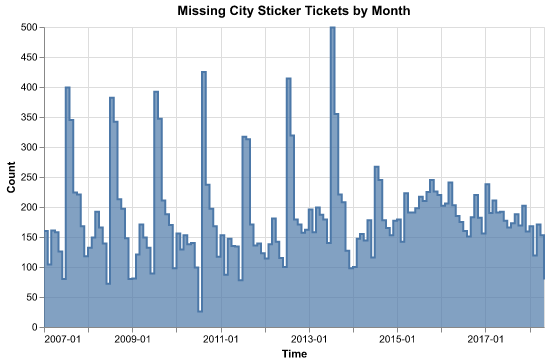
\includegraphics[width=5.73958in,height=3.79167in]{PS2 Answer_files/figure-pdf/cell-7-output-2.png}

\textbf{\emph{Q2}}

\begin{Shaded}
\begin{Highlighting}[]
\CommentTok{\# Find the date of cost increase}
\NormalTok{df\_new\_code }\OperatorTok{=}\NormalTok{ df\_unified[df\_unified[}\StringTok{\textquotesingle{}fine\_level1\_amount\textquotesingle{}}\NormalTok{] }\OperatorTok{==} \DecValTok{200}\NormalTok{]}
\BuiltInTok{print}\NormalTok{(df\_new\_code[}\StringTok{\textquotesingle{}issue\_date\textquotesingle{}}\NormalTok{].iloc[}\DecValTok{0}\NormalTok{])}
\BuiltInTok{print}\NormalTok{(}\StringTok{\textquotesingle{}So we know the date of cost increase was 2012{-}02{-}25.\textquotesingle{}}\NormalTok{)}
\NormalTok{cost\_increase\_date }\OperatorTok{=} \StringTok{\textquotesingle{}2012{-}02{-}25\textquotesingle{}}

\CommentTok{\# Add a vertical line at 2012{-}02{-}25}
\NormalTok{rule }\OperatorTok{=}\NormalTok{ alt.Chart(}
\NormalTok{    pd.DataFrame(}
\NormalTok{        \{}
            \StringTok{\textquotesingle{}cost\_increase\_date\textquotesingle{}}\NormalTok{: [cost\_increase\_date], }
            \StringTok{\textquotesingle{}label\textquotesingle{}}\NormalTok{: [}\StringTok{\textquotesingle{}Cost Increase\textquotesingle{}}\NormalTok{]}
\NormalTok{            \}}
\NormalTok{        )}
\NormalTok{    ).mark\_rule(}
\NormalTok{    color}\OperatorTok{=}\StringTok{\textquotesingle{}red\textquotesingle{}}\NormalTok{,}
\NormalTok{    strokeDash}\OperatorTok{=}\NormalTok{[}\DecValTok{8}\NormalTok{, }\DecValTok{4}\NormalTok{]}
\NormalTok{).encode(}
\NormalTok{    x}\OperatorTok{=}\StringTok{\textquotesingle{}cost\_increase\_date:T\textquotesingle{}}\NormalTok{,}
\NormalTok{    tooltip}\OperatorTok{=}\NormalTok{[}\StringTok{\textquotesingle{}label\textquotesingle{}}\NormalTok{]}
\NormalTok{)}

\CommentTok{\# Label for cost increase}
\NormalTok{text }\OperatorTok{=}\NormalTok{ alt.Chart(}
\NormalTok{    pd.DataFrame(}
\NormalTok{        \{}
            \StringTok{\textquotesingle{}cost\_increase\_date\textquotesingle{}}\NormalTok{: [cost\_increase\_date], }
            \StringTok{\textquotesingle{}label\textquotesingle{}}\NormalTok{: [}\StringTok{\textquotesingle{}2012{-}02{-}25\textquotesingle{}}\NormalTok{]}
\NormalTok{            \}}
\NormalTok{        )}
\NormalTok{    ).mark\_text(}
\NormalTok{    align}\OperatorTok{=}\StringTok{\textquotesingle{}left\textquotesingle{}}\NormalTok{,}
\NormalTok{    baseline}\OperatorTok{=}\StringTok{\textquotesingle{}bottom\textquotesingle{}}\NormalTok{,}
\NormalTok{    dx}\OperatorTok{={-}}\DecValTok{20}\NormalTok{,}
\NormalTok{    dy}\OperatorTok{=}\DecValTok{150}\NormalTok{,}
\NormalTok{    color}\OperatorTok{=}\StringTok{\textquotesingle{}red\textquotesingle{}}
\NormalTok{).encode(}
\NormalTok{    x}\OperatorTok{=}\StringTok{\textquotesingle{}cost\_increase\_date:T\textquotesingle{}}\NormalTok{,}
\NormalTok{    text}\OperatorTok{=}\StringTok{\textquotesingle{}label\textquotesingle{}}
\NormalTok{)}

\NormalTok{chart\_1 }\OperatorTok{+}\NormalTok{ rule }\OperatorTok{+}\NormalTok{ text}
\end{Highlighting}
\end{Shaded}

\begin{verbatim}
2012-02-25 02:00:00
So we know the date of cost increase was 2012-02-25.
\end{verbatim}

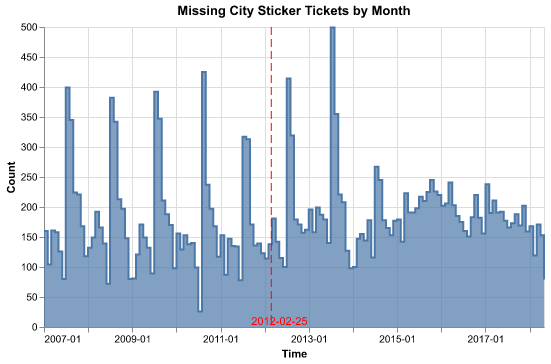
\includegraphics[width=5.73958in,height=3.79167in]{PS2 Answer_files/figure-pdf/cell-8-output-2.png}

\href{https://altair-viz.github.io/user_guide/marks/rule.html\#}{Help
page} (https://altair-viz.github.io/user\_guide/marks/rule.html\#)

\textbf{\emph{Q3}}

\begin{Shaded}
\begin{Highlighting}[]
\CommentTok{\# Filter out data in 2011}
\NormalTok{df\_2011 }\OperatorTok{=}\NormalTok{ df\_unified[df\_unified[}\StringTok{\textquotesingle{}issue\_date\textquotesingle{}}\NormalTok{].dt.year }\OperatorTok{==} \DecValTok{2011}\NormalTok{]}
\NormalTok{tickets\_2011 }\OperatorTok{=}\NormalTok{ df\_2011.shape[}\DecValTok{0}\NormalTok{]}
\BuiltInTok{print}\NormalTok{(}\SpecialStringTok{f\textquotesingle{}}\SpecialCharTok{\{}\NormalTok{tickets\_2011}\SpecialCharTok{\}}\SpecialStringTok{ no city sticker tickets were issued in 2011.\textquotesingle{}}\NormalTok{)}
\CommentTok{\# We assume the same amount later on}
\NormalTok{revenue\_increase }\OperatorTok{=}\NormalTok{ tickets\_2011 }\OperatorTok{*}\NormalTok{ (}\DecValTok{200} \OperatorTok{{-}} \DecValTok{120}\NormalTok{) }\OperatorTok{*} \DecValTok{100} \CommentTok{\# Dataset is one percent}
\BuiltInTok{print}\NormalTok{(revenue\_increase)}
\end{Highlighting}
\end{Shaded}

\begin{verbatim}
1933 no city sticker tickets were issued in 2011.
15464000
\end{verbatim}

So they should have expected \$15464000 of revenue increase, which is
approximately 15.5 million US dollars per year. \newpage
\textbf{\emph{Q4}}

\begin{Shaded}
\begin{Highlighting}[]
\CommentTok{\# Before price increased}
\NormalTok{df\_before\_increase }\OperatorTok{=}\NormalTok{ df\_unified[df\_unified[}\StringTok{\textquotesingle{}fine\_level1\_amount\textquotesingle{}}\NormalTok{] }\OperatorTok{==} \DecValTok{120}\NormalTok{]}
\NormalTok{df\_before\_paid }\OperatorTok{=}\NormalTok{ df\_before\_increase[df\_before\_increase[}\StringTok{\textquotesingle{}ticket\_queue\textquotesingle{}}\NormalTok{] }\OperatorTok{==} \StringTok{\textquotesingle{}Paid\textquotesingle{}}\NormalTok{]}
\NormalTok{paid\_rate\_before }\OperatorTok{=}\NormalTok{ df\_before\_paid.shape[}\DecValTok{0}\NormalTok{] }\OperatorTok{/}\NormalTok{ df\_before\_increase.shape[}\DecValTok{0}\NormalTok{]}
\BuiltInTok{print}\NormalTok{(}\SpecialStringTok{f\textquotesingle{}Before increase, the repayment rate was }\SpecialCharTok{\{}\NormalTok{paid\_rate\_before}\SpecialCharTok{\}}\SpecialStringTok{.\textquotesingle{}}\NormalTok{)}

\CommentTok{\# Filter out data in 2013}
\NormalTok{df\_2013 }\OperatorTok{=}\NormalTok{ df\_unified[df\_unified[}\StringTok{\textquotesingle{}issue\_date\textquotesingle{}}\NormalTok{].dt.year }\OperatorTok{==} \DecValTok{2013}\NormalTok{]}
\NormalTok{df\_2013\_paid }\OperatorTok{=}\NormalTok{ df\_2013[df\_2013[}\StringTok{\textquotesingle{}ticket\_queue\textquotesingle{}}\NormalTok{] }\OperatorTok{==} \StringTok{\textquotesingle{}Paid\textquotesingle{}}\NormalTok{]}
\NormalTok{paid\_rate\_2013 }\OperatorTok{=}\NormalTok{ df\_2013\_paid.shape[}\DecValTok{0}\NormalTok{] }\OperatorTok{/}\NormalTok{ df\_2013.shape[}\DecValTok{0}\NormalTok{]}
\BuiltInTok{print}\NormalTok{(}\SpecialStringTok{f\textquotesingle{}In the calendar year after increase, repayment rate was }\SpecialCharTok{\{}\NormalTok{paid\_rate\_2013}\SpecialCharTok{\}}\SpecialStringTok{.\textquotesingle{}}\NormalTok{)}

\BuiltInTok{print}\NormalTok{(}\StringTok{\textquotesingle{}So we see a drop in repayment rate in tickets after the price was increased.\textquotesingle{}}\NormalTok{)}
\BuiltInTok{print}\NormalTok{(}\StringTok{\textquotesingle{}From around 54\% to 41\%.\textquotesingle{}}\NormalTok{)}

\CommentTok{\# Under repayment rate of 41\%}
\CommentTok{\# We still assume 1933 tickets per year}
\NormalTok{revenue\_increase\_rate }\OperatorTok{=}\NormalTok{ (}
\NormalTok{    tickets\_2011 }\OperatorTok{*}\NormalTok{ paid\_rate\_2013 }\OperatorTok{*} \DecValTok{200} \OperatorTok{{-}}\NormalTok{ tickets\_2011 }\OperatorTok{*}\NormalTok{ paid\_rate\_before }\OperatorTok{*} \DecValTok{120}
\NormalTok{    ) }\OperatorTok{*} \DecValTok{100} 
\BuiltInTok{print}\NormalTok{(revenue\_increase\_rate)}
\end{Highlighting}
\end{Shaded}

\begin{verbatim}
Before increase, the repayment rate was 0.5431306934374419.
In the calendar year after increase, repayment rate was 0.4059213089209194.
So we see a drop in repayment rate in tickets after the price was increased.
From around 54% to 41%.
3094458.2379078404
\end{verbatim}

Under the new repayment rates, the change in revenue should have been
about approximately 3.1 million US dollars per year.

\textbf{\emph{Q5}}

\begin{Shaded}
\begin{Highlighting}[]
\CommentTok{\# Again use the dataframe aggregated by month and year}
\CommentTok{\# We already have total tickets for each month{-}year in the previous question}
\CommentTok{\# Now we only need to count paid tickets}
\NormalTok{df\_paid }\OperatorTok{=}\NormalTok{ df\_unified[df\_unified[}\StringTok{\textquotesingle{}ticket\_queue\textquotesingle{}}\NormalTok{] }\OperatorTok{==} \StringTok{\textquotesingle{}Paid\textquotesingle{}}\NormalTok{]}
\NormalTok{group\_paid }\OperatorTok{=}\NormalTok{ df\_paid.groupby(}\StringTok{\textquotesingle{}issue\_y\_m\textquotesingle{}}\NormalTok{)}
\NormalTok{df\_paid\_count }\OperatorTok{=}\NormalTok{ group\_paid.size().reset\_index(name}\OperatorTok{=}\StringTok{\textquotesingle{}count\_paid\textquotesingle{}}\NormalTok{)}

\CommentTok{\# Combine with the count of total tickets}
\NormalTok{Q5\_count }\OperatorTok{=}\NormalTok{ pd.merge(df\_paid\_count, Q1\_count)}
\CommentTok{\# Calculate repayment rates in a new column}
\NormalTok{Q5\_count[}\StringTok{\textquotesingle{}repayment\_rate\textquotesingle{}}\NormalTok{] }\OperatorTok{=}\NormalTok{ Q5\_count[}\StringTok{\textquotesingle{}count\_paid\textquotesingle{}}\NormalTok{] }\OperatorTok{/}\NormalTok{ Q5\_count[}\StringTok{\textquotesingle{}count\textquotesingle{}}\NormalTok{]}
\BuiltInTok{print}\NormalTok{(Q5\_count.head(}\DecValTok{10}\NormalTok{)) }\CommentTok{\# Ready for plotting}

\NormalTok{chart2 }\OperatorTok{=}\NormalTok{ alt.Chart(Q5\_count).mark\_line().encode(}
\NormalTok{    alt.X(}\StringTok{\textquotesingle{}issue\_y\_m:T\textquotesingle{}}\NormalTok{, title}\OperatorTok{=}\StringTok{\textquotesingle{}Time\textquotesingle{}}\NormalTok{, axis}\OperatorTok{=}\NormalTok{alt.Axis(}\BuiltInTok{format}\OperatorTok{=}\StringTok{\textquotesingle{}\%Y{-}\%m\textquotesingle{}}\NormalTok{)),}
\NormalTok{    alt.Y(}\StringTok{\textquotesingle{}repayment\_rate:Q\textquotesingle{}}\NormalTok{, title}\OperatorTok{=}\StringTok{\textquotesingle{}Repayment Rates\textquotesingle{}}\NormalTok{)}
\NormalTok{).properties(}
\NormalTok{    width}\OperatorTok{=}\DecValTok{500}\NormalTok{,}
\NormalTok{    title}\OperatorTok{=}\StringTok{\textquotesingle{}Repayment Rates of No City Sticker Tickets by Month\textquotesingle{}}
\NormalTok{)}

\CommentTok{\# The verticle line and annotation have been set in Question 2.}
\NormalTok{chart2 }\OperatorTok{+}\NormalTok{ rule }\OperatorTok{+}\NormalTok{ text}
\end{Highlighting}
\end{Shaded}

\begin{verbatim}
  issue_y_m  count_paid  count  repayment_rate
0   2007-01          85    160        0.531250
1   2007-02          55    104        0.528846
2   2007-03          90    161        0.559006
3   2007-04          83    158        0.525316
4   2007-05          66    126        0.523810
5   2007-06          48     80        0.600000
6   2007-07         255    399        0.639098
7   2007-08         198    345        0.573913
8   2007-09         115    224        0.513393
9   2007-10         115    221        0.520362
\end{verbatim}

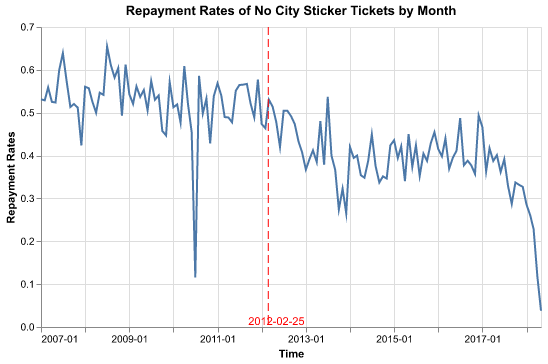
\includegraphics[width=5.70833in,height=3.79167in]{PS2 Answer_files/figure-pdf/cell-11-output-2.png}

From the plot, we can see a downward trend in repayment rates of no city
sticker tickets over time, after the new policy was introduced. The
repayment rates kept fluctuating, but after the price went up, repayment
rates were in general significantly lower than before. The average level
under the new policy was apparently below that under the old code.
Moreover, toward the end of our dataset, there was an ongoing sharp
decline in repayment rates. The rates dropped to extremely low by 2018.

This indicates the need to balance repayment rates and penalty amounts,
in order to boost the government revenue.

\textbf{\emph{Q6}}

\begin{Shaded}
\begin{Highlighting}[]
\CommentTok{\# 000 represents no city sticker}
\NormalTok{df\_Q6 }\OperatorTok{=}\NormalTok{ df.copy()}
\NormalTok{df\_Q6 }\OperatorTok{=}\NormalTok{ df\_Q6.replace(}\StringTok{\textquotesingle{}0964125\textquotesingle{}}\NormalTok{, }\StringTok{\textquotesingle{}000\textquotesingle{}}\NormalTok{)}
\NormalTok{df\_Q6 }\OperatorTok{=}\NormalTok{ df\_Q6.replace(}\StringTok{\textquotesingle{}0964125B\textquotesingle{}}\NormalTok{, }\StringTok{\textquotesingle{}000\textquotesingle{}}\NormalTok{)}

\CommentTok{\# Filter out records before policy change}
\NormalTok{df\_Q6[}\StringTok{\textquotesingle{}issue\_date\textquotesingle{}}\NormalTok{] }\OperatorTok{=}\NormalTok{ pd.to\_datetime(df\_Q6[}\StringTok{\textquotesingle{}issue\_date\textquotesingle{}}\NormalTok{])}
\NormalTok{df\_Q6 }\OperatorTok{=}\NormalTok{ df\_Q6[df\_Q6[}\StringTok{\textquotesingle{}issue\_date\textquotesingle{}}\NormalTok{] }\OperatorTok{\textless{}} \StringTok{\textquotesingle{}2012{-}02{-}25\textquotesingle{}}\NormalTok{]}

\CommentTok{\# Calculate repayment rates}
\NormalTok{grouped\_code }\OperatorTok{=}\NormalTok{ df\_Q6.groupby(}\StringTok{\textquotesingle{}violation\_code\textquotesingle{}}\NormalTok{)}
\NormalTok{df\_code\_count }\OperatorTok{=}\NormalTok{ grouped\_code.size().reset\_index(name}\OperatorTok{=}\StringTok{\textquotesingle{}total\_tickets\textquotesingle{}}\NormalTok{)}
\CommentTok{\# Those never paid are ignored here, they are missed in filter and merge}
\CommentTok{\# Never paid tickets are of no relevance}
\NormalTok{df\_Q6\_paid }\OperatorTok{=}\NormalTok{ df\_Q6[df\_Q6[}\StringTok{\textquotesingle{}ticket\_queue\textquotesingle{}}\NormalTok{] }\OperatorTok{==} \StringTok{\textquotesingle{}Paid\textquotesingle{}}\NormalTok{]}
\NormalTok{grouped\_code\_paid }\OperatorTok{=}\NormalTok{ df\_Q6\_paid.groupby(}\StringTok{\textquotesingle{}violation\_code\textquotesingle{}}\NormalTok{)}
\NormalTok{df\_code\_count\_paid }\OperatorTok{=}\NormalTok{ grouped\_code\_paid.size().reset\_index(name}\OperatorTok{=}\StringTok{\textquotesingle{}paid\_tickets\textquotesingle{}}\NormalTok{)}

\NormalTok{Q6\_count }\OperatorTok{=}\NormalTok{ pd.merge(df\_code\_count, df\_code\_count\_paid)}
\NormalTok{Q6\_count[}\StringTok{\textquotesingle{}repayment\_rates\textquotesingle{}}\NormalTok{] }\OperatorTok{=}\NormalTok{ Q6\_count[}\StringTok{\textquotesingle{}paid\_tickets\textquotesingle{}}\NormalTok{] }\OperatorTok{/}\NormalTok{ Q6\_count[}\StringTok{\textquotesingle{}total\_tickets\textquotesingle{}}\NormalTok{]}
\CommentTok{\# We have both ticket counts and repayment rates }

\CommentTok{\# Explore the dataset: tickets issued}
\NormalTok{Q6\_count }\OperatorTok{=}\NormalTok{ Q6\_count.sort\_values(by}\OperatorTok{=}\StringTok{\textquotesingle{}total\_tickets\textquotesingle{}}\NormalTok{, ascending}\OperatorTok{=}\VariableTok{False}\NormalTok{)}
\BuiltInTok{print}\NormalTok{(Q6\_count.head(}\DecValTok{15}\NormalTok{))}
\end{Highlighting}
\end{Shaded}

\begin{verbatim}
   violation_code  total_tickets  paid_tickets  repayment_rates
74       0976160F          22545         13743         0.609581
51        0964190          18756         15124         0.806355
10       0964040B          14740         12037         0.816621
20       0964090E          11683          8897         0.761534
0             000          10758          5843         0.543131
43       0964150B           9883          7186         0.727107
70       0976160A           8531          5166         0.605556
18       0964080A           7269          5696         0.783602
19       0964080B           3547          2733         0.770510
52       0964190A           3504          2952         0.842466
41       0964140B           3354          2341         0.697973
23       0964100A           3042          2141         0.703813
46       0964170A           2440          1756         0.719672
40        0964130           1643           844         0.513694
30       0964110A           1431           918         0.641509
\end{verbatim}

The suggested three violation types would be 0964190 (`EXPIRED METER OR
OVERSTAY'), 0964040B (`STREET CLEANING'), and 0976160F (`EXPIRED PLATES
OR TEMPORARY REGISTRATION').

This is because we need to seek for both high total number of tickets
and high repayment rates. We use the multiplication of these two
parameters as measure, which is paid\_tickets. From the dataframe
Q6\_count as shown above, we could tell that these three violation codes
have relatively higher total\_ticket counts and repayment rates. They
have the most paid tickets in 2011.

\begin{Shaded}
\begin{Highlighting}[]
\CommentTok{\# To boost revenue, the amount of tickets should be large to make a difference.}
\CommentTok{\# By inspection, we set the bar of 5000 total tickets in 2011 here.}
\NormalTok{Q6\_count }\OperatorTok{=}\NormalTok{ Q6\_count[Q6\_count[}\StringTok{\textquotesingle{}total\_tickets\textquotesingle{}}\NormalTok{] }\OperatorTok{\textgreater{}} \DecValTok{5000}\NormalTok{]}

\NormalTok{chart\_3 }\OperatorTok{=}\NormalTok{ alt.Chart(Q6\_count).mark\_circle(size}\OperatorTok{=}\DecValTok{200}\NormalTok{).encode(}
\NormalTok{    alt.X(}\StringTok{\textquotesingle{}total\_tickets:Q\textquotesingle{}}\NormalTok{, title}\OperatorTok{=}\StringTok{\textquotesingle{}Tickets Issued\textquotesingle{}}\NormalTok{).scale(zero}\OperatorTok{=}\VariableTok{False}\NormalTok{),}
\NormalTok{    alt.Y(}\StringTok{\textquotesingle{}repayment\_rates:Q\textquotesingle{}}\NormalTok{, title}\OperatorTok{=}\StringTok{\textquotesingle{}Repayment Rates\textquotesingle{}}\NormalTok{).scale(zero}\OperatorTok{=}\VariableTok{False}\NormalTok{),}
\NormalTok{    color}\OperatorTok{=}\StringTok{\textquotesingle{}violation\_code:N\textquotesingle{}}\NormalTok{).properties(}
\NormalTok{    width}\OperatorTok{=}\DecValTok{500}\NormalTok{,}
\NormalTok{    title}\OperatorTok{=}\StringTok{\textquotesingle{}Ticket Counts and Repayment Rates of Top Violation Types in 2011\textquotesingle{}}
\NormalTok{)}

\NormalTok{chart\_3}
\end{Highlighting}
\end{Shaded}

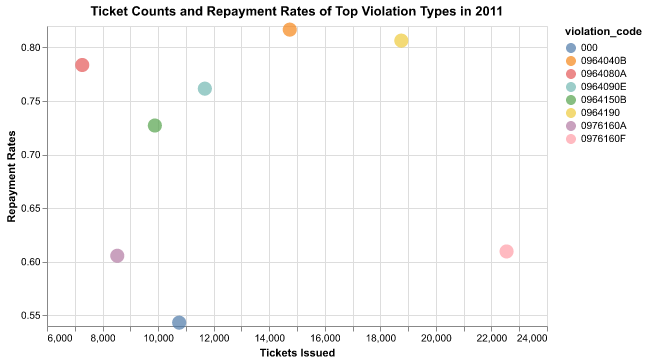
\includegraphics[width=6.75in,height=3.78125in]{PS2 Answer_files/figure-pdf/cell-13-output-1.png}

The plot supports the argument by providing a contrast among different
violation codes. The three dots we chose, 0964190, 0976160F, 0964040B,
are positioned either high on the y-axis, indicating higher repayment
rates, or far to the right on the x-axis, representing a larger number
of tickets issued, or both. In this plot, we could find 0964190,
0976160F, 0964040B might be the three best choices. \newpage

\subsection{Headlines and
sub-messages}\label{headlines-and-sub-messages}

\textbf{\emph{Q1}}

\begin{Shaded}
\begin{Highlighting}[]
\NormalTok{grouped\_description }\OperatorTok{=}\NormalTok{ df.groupby(}\StringTok{\textquotesingle{}violation\_description\textquotesingle{}}\NormalTok{)}

\CommentTok{\# Description and repayment rate}
\NormalTok{total\_count }\OperatorTok{=}\NormalTok{ grouped\_description.size().reset\_index(name}\OperatorTok{=}\StringTok{\textquotesingle{}total\_tickets\textquotesingle{}}\NormalTok{)}

\NormalTok{df\_paid }\OperatorTok{=}\NormalTok{ df[df[}\StringTok{\textquotesingle{}ticket\_queue\textquotesingle{}}\NormalTok{] }\OperatorTok{==} \StringTok{\textquotesingle{}Paid\textquotesingle{}}\NormalTok{].copy()}
\NormalTok{grouped\_des\_paid }\OperatorTok{=}\NormalTok{ df\_paid.groupby(}\StringTok{\textquotesingle{}violation\_description\textquotesingle{}}\NormalTok{)}
\NormalTok{paid\_count }\OperatorTok{=}\NormalTok{ grouped\_des\_paid.size().reset\_index(name}\OperatorTok{=}\StringTok{\textquotesingle{}paid\_tickets\textquotesingle{}}\NormalTok{)}

\CommentTok{\# Those left out in df\_paid are violation never paid}
\NormalTok{all\_violations }\OperatorTok{=}\NormalTok{ df[}\StringTok{\textquotesingle{}violation\_description\textquotesingle{}}\NormalTok{].unique()}
\NormalTok{paid\_violations }\OperatorTok{=}\NormalTok{ df\_paid[}\StringTok{\textquotesingle{}violation\_description\textquotesingle{}}\NormalTok{].unique()}
\NormalTok{unpaid\_violations }\OperatorTok{=}\NormalTok{ [item }\ControlFlowTok{for}\NormalTok{ item }\KeywordTok{in}\NormalTok{ all\_violations }\ControlFlowTok{if}\NormalTok{ item }\KeywordTok{not} \KeywordTok{in}\NormalTok{ paid\_violations]}
\CommentTok{\# Fill in with 0 paid tickets for these three types}
\NormalTok{unpaid\_dict }\OperatorTok{=}\NormalTok{ \{}
    \StringTok{\textquotesingle{}violation\_description\textquotesingle{}}\NormalTok{: unpaid\_violations, }
    \StringTok{\textquotesingle{}paid\_tickets\textquotesingle{}}\NormalTok{: [}\DecValTok{0}\NormalTok{, }\DecValTok{0}\NormalTok{, }\DecValTok{0}\NormalTok{]}
\NormalTok{    \}}
\NormalTok{unpaid\_df }\OperatorTok{=}\NormalTok{ pd.DataFrame(unpaid\_dict)}
\NormalTok{paid\_count }\OperatorTok{=}\NormalTok{ pd.concat([paid\_count, unpaid\_df], ignore\_index}\OperatorTok{=}\VariableTok{True}\NormalTok{)}

\NormalTok{description\_payment }\OperatorTok{=}\NormalTok{ pd.merge(}
\NormalTok{    total\_count, paid\_count, }
\NormalTok{    on}\OperatorTok{=}\StringTok{\textquotesingle{}violation\_description\textquotesingle{}}
\NormalTok{    )}
\NormalTok{description\_payment[}\StringTok{\textquotesingle{}repayment\_rates\textquotesingle{}}\NormalTok{] }\OperatorTok{=}\NormalTok{ description\_payment[}\StringTok{\textquotesingle{}paid\_tickets\textquotesingle{}}\NormalTok{] }\OperatorTok{/} \OperatorTok{\textbackslash{}}
\NormalTok{                                         description\_payment[}\StringTok{\textquotesingle{}total\_tickets\textquotesingle{}}\NormalTok{]}

\CommentTok{\# Description and average fine amount}
\NormalTok{description\_price }\OperatorTok{=}\NormalTok{ grouped\_description[}\StringTok{\textquotesingle{}fine\_level1\_amount\textquotesingle{}}\NormalTok{].mean()}
\NormalTok{description\_price }\OperatorTok{=}\NormalTok{ description\_price.reset\_index(name}\OperatorTok{=}\StringTok{\textquotesingle{}avg\_price\textquotesingle{}}\NormalTok{)}

\NormalTok{description\_summary }\OperatorTok{=}\NormalTok{ pd.merge(description\_payment, description\_price)}

\CommentTok{\# Sort by frequency and print most common 5}
\NormalTok{Q\_3\_1 }\OperatorTok{=}\NormalTok{ description\_summary.sort\_values(}\StringTok{\textquotesingle{}total\_tickets\textquotesingle{}}\NormalTok{, ascending}\OperatorTok{=}\VariableTok{False}\NormalTok{)}
\NormalTok{Q\_3\_1 }\OperatorTok{=}\NormalTok{ Q\_3\_1[[}\StringTok{\textquotesingle{}violation\_description\textquotesingle{}}\NormalTok{, }\StringTok{\textquotesingle{}repayment\_rates\textquotesingle{}}\NormalTok{, }\StringTok{\textquotesingle{}avg\_price\textquotesingle{}}\NormalTok{]]}
\BuiltInTok{print}\NormalTok{(Q\_3\_1.head(}\DecValTok{5}\NormalTok{))}
\end{Highlighting}
\end{Shaded}

\begin{verbatim}
                        violation_description  repayment_rates  avg_price
23   EXPIRED PLATES OR TEMPORARY REGISTRATION         0.604361  54.968869
101                           STREET CLEANING         0.811612  54.004249
90                 RESIDENTIAL PERMIT PARKING         0.742262  66.338302
19   EXP. METER NON-CENTRAL BUSINESS DISTRICT         0.792913  46.598058
81        PARKING/STANDING PROHIBITED ANYTIME         0.705817  66.142864
\end{verbatim}

\textbf{\emph{Q2}}

\begin{Shaded}
\begin{Highlighting}[]
\CommentTok{\# Filter out types more than 100 times }
\NormalTok{Q\_3\_2 }\OperatorTok{=}\NormalTok{ description\_summary[description\_summary[}\StringTok{\textquotesingle{}total\_tickets\textquotesingle{}}\NormalTok{] }\OperatorTok{\textgreater{}} \DecValTok{99}\NormalTok{]}

\CommentTok{\# Exclude the extreme value with high fine amount}
\BuiltInTok{print}\NormalTok{(Q\_3\_2.sort\_values(}\StringTok{\textquotesingle{}avg\_price\textquotesingle{}}\NormalTok{, ascending}\OperatorTok{=}\VariableTok{False}\NormalTok{)[}\DecValTok{0}\NormalTok{: }\DecValTok{5}\NormalTok{])}
\BuiltInTok{print}\NormalTok{(}\StringTok{\textquotesingle{}So we need to exclude NO CITY STICKER VEHICLE OVER 16,000 LBS.\textquotesingle{}}\NormalTok{)}
\NormalTok{Q\_3\_2 }\OperatorTok{=}\NormalTok{ Q\_3\_2[Q\_3\_2[}\StringTok{\textquotesingle{}violation\_description\textquotesingle{}}\NormalTok{] }\OperatorTok{!=} \StringTok{\textquotesingle{}NO CITY STICKER VEHICLE OVER 16,000 LBS.\textquotesingle{}}\NormalTok{]}

\CommentTok{\# Scatter plot}
\NormalTok{chart\_4 }\OperatorTok{=}\NormalTok{ alt.Chart(Q\_3\_2).mark\_point().encode(}
\NormalTok{    alt.X(}\StringTok{\textquotesingle{}avg\_price:Q\textquotesingle{}}\NormalTok{, title}\OperatorTok{=}\StringTok{\textquotesingle{}Average Fine Amount\textquotesingle{}}\NormalTok{),}
\NormalTok{    alt.Y(}\StringTok{\textquotesingle{}repayment\_rates:Q\textquotesingle{}}\NormalTok{, title}\OperatorTok{=}\StringTok{\textquotesingle{}Repayment Rates\textquotesingle{}}\NormalTok{)}
\NormalTok{).properties(}
\NormalTok{    title}\OperatorTok{=}\StringTok{\textquotesingle{}Average Fine Amount Versus Repayment Rates\textquotesingle{}}
\NormalTok{)}

\NormalTok{chart\_4}
\end{Highlighting}
\end{Shaded}

\begin{verbatim}
                                violation_description  total_tickets  \
42           NO CITY STICKER VEHICLE OVER 16,000 LBS.            131   
15                              DISABLED PARKING ZONE           2034   
43  NO CITY STICKER VEHICLE UNDER/EQUAL TO 16,000 ...          14246   
54            OBSTRUCTED OR IMPROPERLY TINTED WINDOWS            271   
95              SMOKED/TINTED WINDOWS PARKED/STANDING           1697   

    paid_tickets  repayment_rates   avg_price  
42            16         0.122137  500.000000  
15          1102         0.541790  216.986234  
43          5675         0.398357  200.000000  
54           150         0.553506  156.180812  
95          1060         0.624632  151.090159  
So we need to exclude NO CITY STICKER VEHICLE OVER 16,000 LBS.
\end{verbatim}

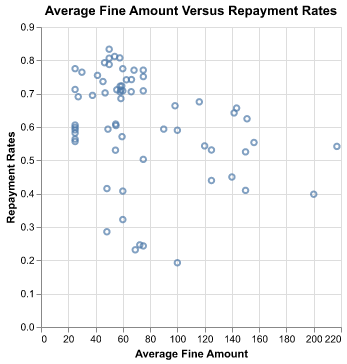
\includegraphics[width=3.61458in,height=3.79167in]{PS2 Answer_files/figure-pdf/cell-15-output-2.png}

Headline: In general, average fine amount and repayment rates are
negatively correlated. As average fine amount goes up, repayment rates
tend to decrease, among top violation types.

Submessages: Most top violation types are priced under \$100 at the
initial stage, with repayment rates ranging from 50\% to 80\%. The
lowest repayment rate is around 20\%, and the lowest average price is
over \$20. The highest repayment rate reaches about 85\%, with an
average fine around \$50. And as average fine amount increases, the
spread of repayment rates becomes more dispersed at first, and then more
condensed.

\begin{Shaded}
\begin{Highlighting}[]
\NormalTok{chart\_5 }\OperatorTok{=}\NormalTok{ alt.Chart(Q\_3\_2).mark\_bar().encode(}
\NormalTok{    alt.X(}
        \StringTok{\textquotesingle{}avg\_price:Q\textquotesingle{}}\NormalTok{, }
\NormalTok{        title}\OperatorTok{=}\StringTok{\textquotesingle{}Average Fine Amount\textquotesingle{}}\NormalTok{, }
        \BuiltInTok{bin}\OperatorTok{=}\NormalTok{alt.BinParams(maxbins}\OperatorTok{=}\DecValTok{20}\NormalTok{)}
\NormalTok{        ),}
\NormalTok{    alt.Y(}
        \StringTok{\textquotesingle{}repayment\_rates:Q\textquotesingle{}}\NormalTok{, }
\NormalTok{        title}\OperatorTok{=}\StringTok{\textquotesingle{}Repayment Rates\textquotesingle{}}\NormalTok{, }
        \BuiltInTok{bin}\OperatorTok{=}\NormalTok{alt.BinParams(maxbins}\OperatorTok{=}\DecValTok{20}\NormalTok{)}
\NormalTok{        ),}
\NormalTok{    alt.Color(}\StringTok{\textquotesingle{}count()\textquotesingle{}}\NormalTok{)}
\NormalTok{).properties(}
\NormalTok{    title}\OperatorTok{=}\StringTok{\textquotesingle{}Average Fine Amount Versus Repayment Rates\textquotesingle{}}
\NormalTok{)}

\NormalTok{chart\_5}
\end{Highlighting}
\end{Shaded}

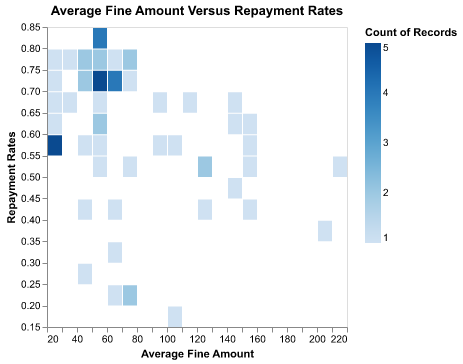
\includegraphics[width=4.82292in,height=3.79167in]{PS2 Answer_files/figure-pdf/cell-16-output-1.png}

Headline: Most of frequent violation types are priced between \$20 and
\$80, with repayment rates ranging from 55\% and 85\%.

Submessages: Repayment rates tend to decrease with increase in average
fine amount when we focus on most frequent violation types. Besides, as
average penalty amount goes up, the range of repayment rates gets wider
abd then narrower, finally concentrated at a more consistent yet lower
level.

\begin{Shaded}
\begin{Highlighting}[]
\NormalTok{chart\_6 }\OperatorTok{=}\NormalTok{ alt.Chart(Q\_3\_2).mark\_boxplot().encode(}
\NormalTok{    alt.X(}
        \StringTok{\textquotesingle{}avg\_price:Q\textquotesingle{}}\NormalTok{, }
\NormalTok{        title}\OperatorTok{=}\StringTok{\textquotesingle{}Average Fine Amount\textquotesingle{}}\NormalTok{, }
        \BuiltInTok{bin}\OperatorTok{=}\NormalTok{alt.BinParams(maxbins}\OperatorTok{=}\DecValTok{20}\NormalTok{)}
\NormalTok{        ),}
\NormalTok{    alt.Y(}
        \StringTok{\textquotesingle{}repayment\_rates:Q\textquotesingle{}}\NormalTok{, }
\NormalTok{        title}\OperatorTok{=}\StringTok{\textquotesingle{}Repayment Rates\textquotesingle{}}
\NormalTok{        )}
\NormalTok{).properties(}
\NormalTok{    title}\OperatorTok{=}\StringTok{\textquotesingle{}Average Fine Amount Versus Repayment Rates\textquotesingle{}}
\NormalTok{)}

\NormalTok{chart\_6 }
\end{Highlighting}
\end{Shaded}

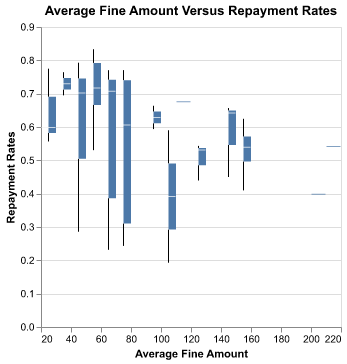
\includegraphics[width=3.61458in,height=3.79167in]{PS2 Answer_files/figure-pdf/cell-17-output-1.png}

Headline: With the increase in average price, the spread of repayment
rates widens and then narrows.

Submessages: There is a concave trend in the median of repaymemt rates
as average fine amount goes up. Among top violation types, few records
exist when the average price exceeds \$160. And in general, repayment
rates decrease when average fine amount increases.

\textbf{\emph{Q3}}

The first plot, scatter plot, would be the best choice because it shows
every single violation type, in a very direct and straightforward way.
Readers can follow the dots and identify the genreal trend at first
sight without additional information. They could easily tell that as
average fine amount goes up, repayment ratea tend to decline.

By contrast, other two plots require some effort in understanding the
meaning of squares and dots or some knowledge of statistical concepts
such as quartile and bins.

\subsection{Understanding the structure of the data and summarizing
it}\label{understanding-the-structure-of-the-data-and-summarizing-it}

\textbf{\emph{Q1}}

\begin{Shaded}
\begin{Highlighting}[]
\CommentTok{\# Filter out records unpaid yet price not doubled}
\NormalTok{df\_unpaid }\OperatorTok{=}\NormalTok{ df[df[}\StringTok{\textquotesingle{}ticket\_queue\textquotesingle{}}\NormalTok{] }\OperatorTok{!=} \StringTok{\textquotesingle{}Paid\textquotesingle{}}\NormalTok{]}
\NormalTok{df\_undoubled }\OperatorTok{=}\NormalTok{ df\_unpaid[}
\NormalTok{    df\_unpaid[}\StringTok{\textquotesingle{}fine\_level2\_amount\textquotesingle{}}\NormalTok{] }\OperatorTok{!=}\NormalTok{ df\_unpaid[}\StringTok{\textquotesingle{}fine\_level1\_amount\textquotesingle{}}\NormalTok{] }\OperatorTok{*} \DecValTok{2}
\NormalTok{]}
\BuiltInTok{print}\NormalTok{(}\StringTok{\textquotesingle{}This dataframe is not empty.\textquotesingle{}}\NormalTok{)}
\BuiltInTok{print}\NormalTok{(}\StringTok{\textquotesingle{}So this argument does not hold for all violations.\textquotesingle{}}\NormalTok{)}

\CommentTok{\# Fetch violation types with at least 100 citations}
\NormalTok{Q\_4\_1 }\OperatorTok{=}\NormalTok{ df\_undoubled.groupby(}
    \StringTok{\textquotesingle{}violation\_description\textquotesingle{}}
\NormalTok{    ).size().reset\_index(name}\OperatorTok{=}\StringTok{\textquotesingle{}citation\textquotesingle{}}\NormalTok{)}
\NormalTok{type\_undoubled }\OperatorTok{=}\NormalTok{ Q\_4\_1[}\StringTok{\textquotesingle{}violation\_description\textquotesingle{}}\NormalTok{][Q\_4\_1[}\StringTok{\textquotesingle{}citation\textquotesingle{}}\NormalTok{] }\OperatorTok{\textgreater{}} \DecValTok{99}\NormalTok{].to\_list()}

\NormalTok{df\_undoubled }\OperatorTok{=}\NormalTok{ df\_undoubled[}
\NormalTok{    df\_undoubled[}\StringTok{\textquotesingle{}violation\_description\textquotesingle{}}\NormalTok{].isin(type\_undoubled)}
\NormalTok{    ]}

\NormalTok{df\_diff }\OperatorTok{=}\NormalTok{ df\_undoubled.groupby(}\StringTok{\textquotesingle{}violation\_description\textquotesingle{}}\NormalTok{)}\OperatorTok{\textbackslash{}}
\NormalTok{    [[}\StringTok{\textquotesingle{}fine\_level1\_amount\textquotesingle{}}\NormalTok{, }\StringTok{\textquotesingle{}fine\_level2\_amount\textquotesingle{}}\NormalTok{]].mean().reset\_index()}
\NormalTok{df\_diff[}\StringTok{\textquotesingle{}price\_increase\textquotesingle{}}\NormalTok{] }\OperatorTok{=} \OperatorTok{\textbackslash{}}
\NormalTok{    df\_diff[}\StringTok{\textquotesingle{}fine\_level2\_amount\textquotesingle{}}\NormalTok{] }\OperatorTok{{-}}\NormalTok{ df\_diff[}\StringTok{\textquotesingle{}fine\_level1\_amount\textquotesingle{}}\NormalTok{]}
\BuiltInTok{print}\NormalTok{(}\StringTok{\textquotesingle{}Each ticket increase if unpaid: \textquotesingle{}}\NormalTok{)}
\BuiltInTok{print}\NormalTok{(df\_diff[[}\StringTok{\textquotesingle{}violation\_description\textquotesingle{}}\NormalTok{, }\StringTok{\textquotesingle{}price\_increase\textquotesingle{}}\NormalTok{]])}
\end{Highlighting}
\end{Shaded}

\begin{verbatim}
This dataframe is not empty.
So this argument does not hold for all violations.
Each ticket increase if unpaid: 
                   violation_description  price_increase
0   BLOCK ACCESS/ALLEY/DRIVEWAY/FIRELANE           100.0
1                  DISABLED PARKING ZONE            50.0
2                    PARK OR BLOCK ALLEY           100.0
3  SMOKED/TINTED WINDOWS PARKED/STANDING             0.0
\end{verbatim}

\newpage

\textbf{\emph{Q2}}
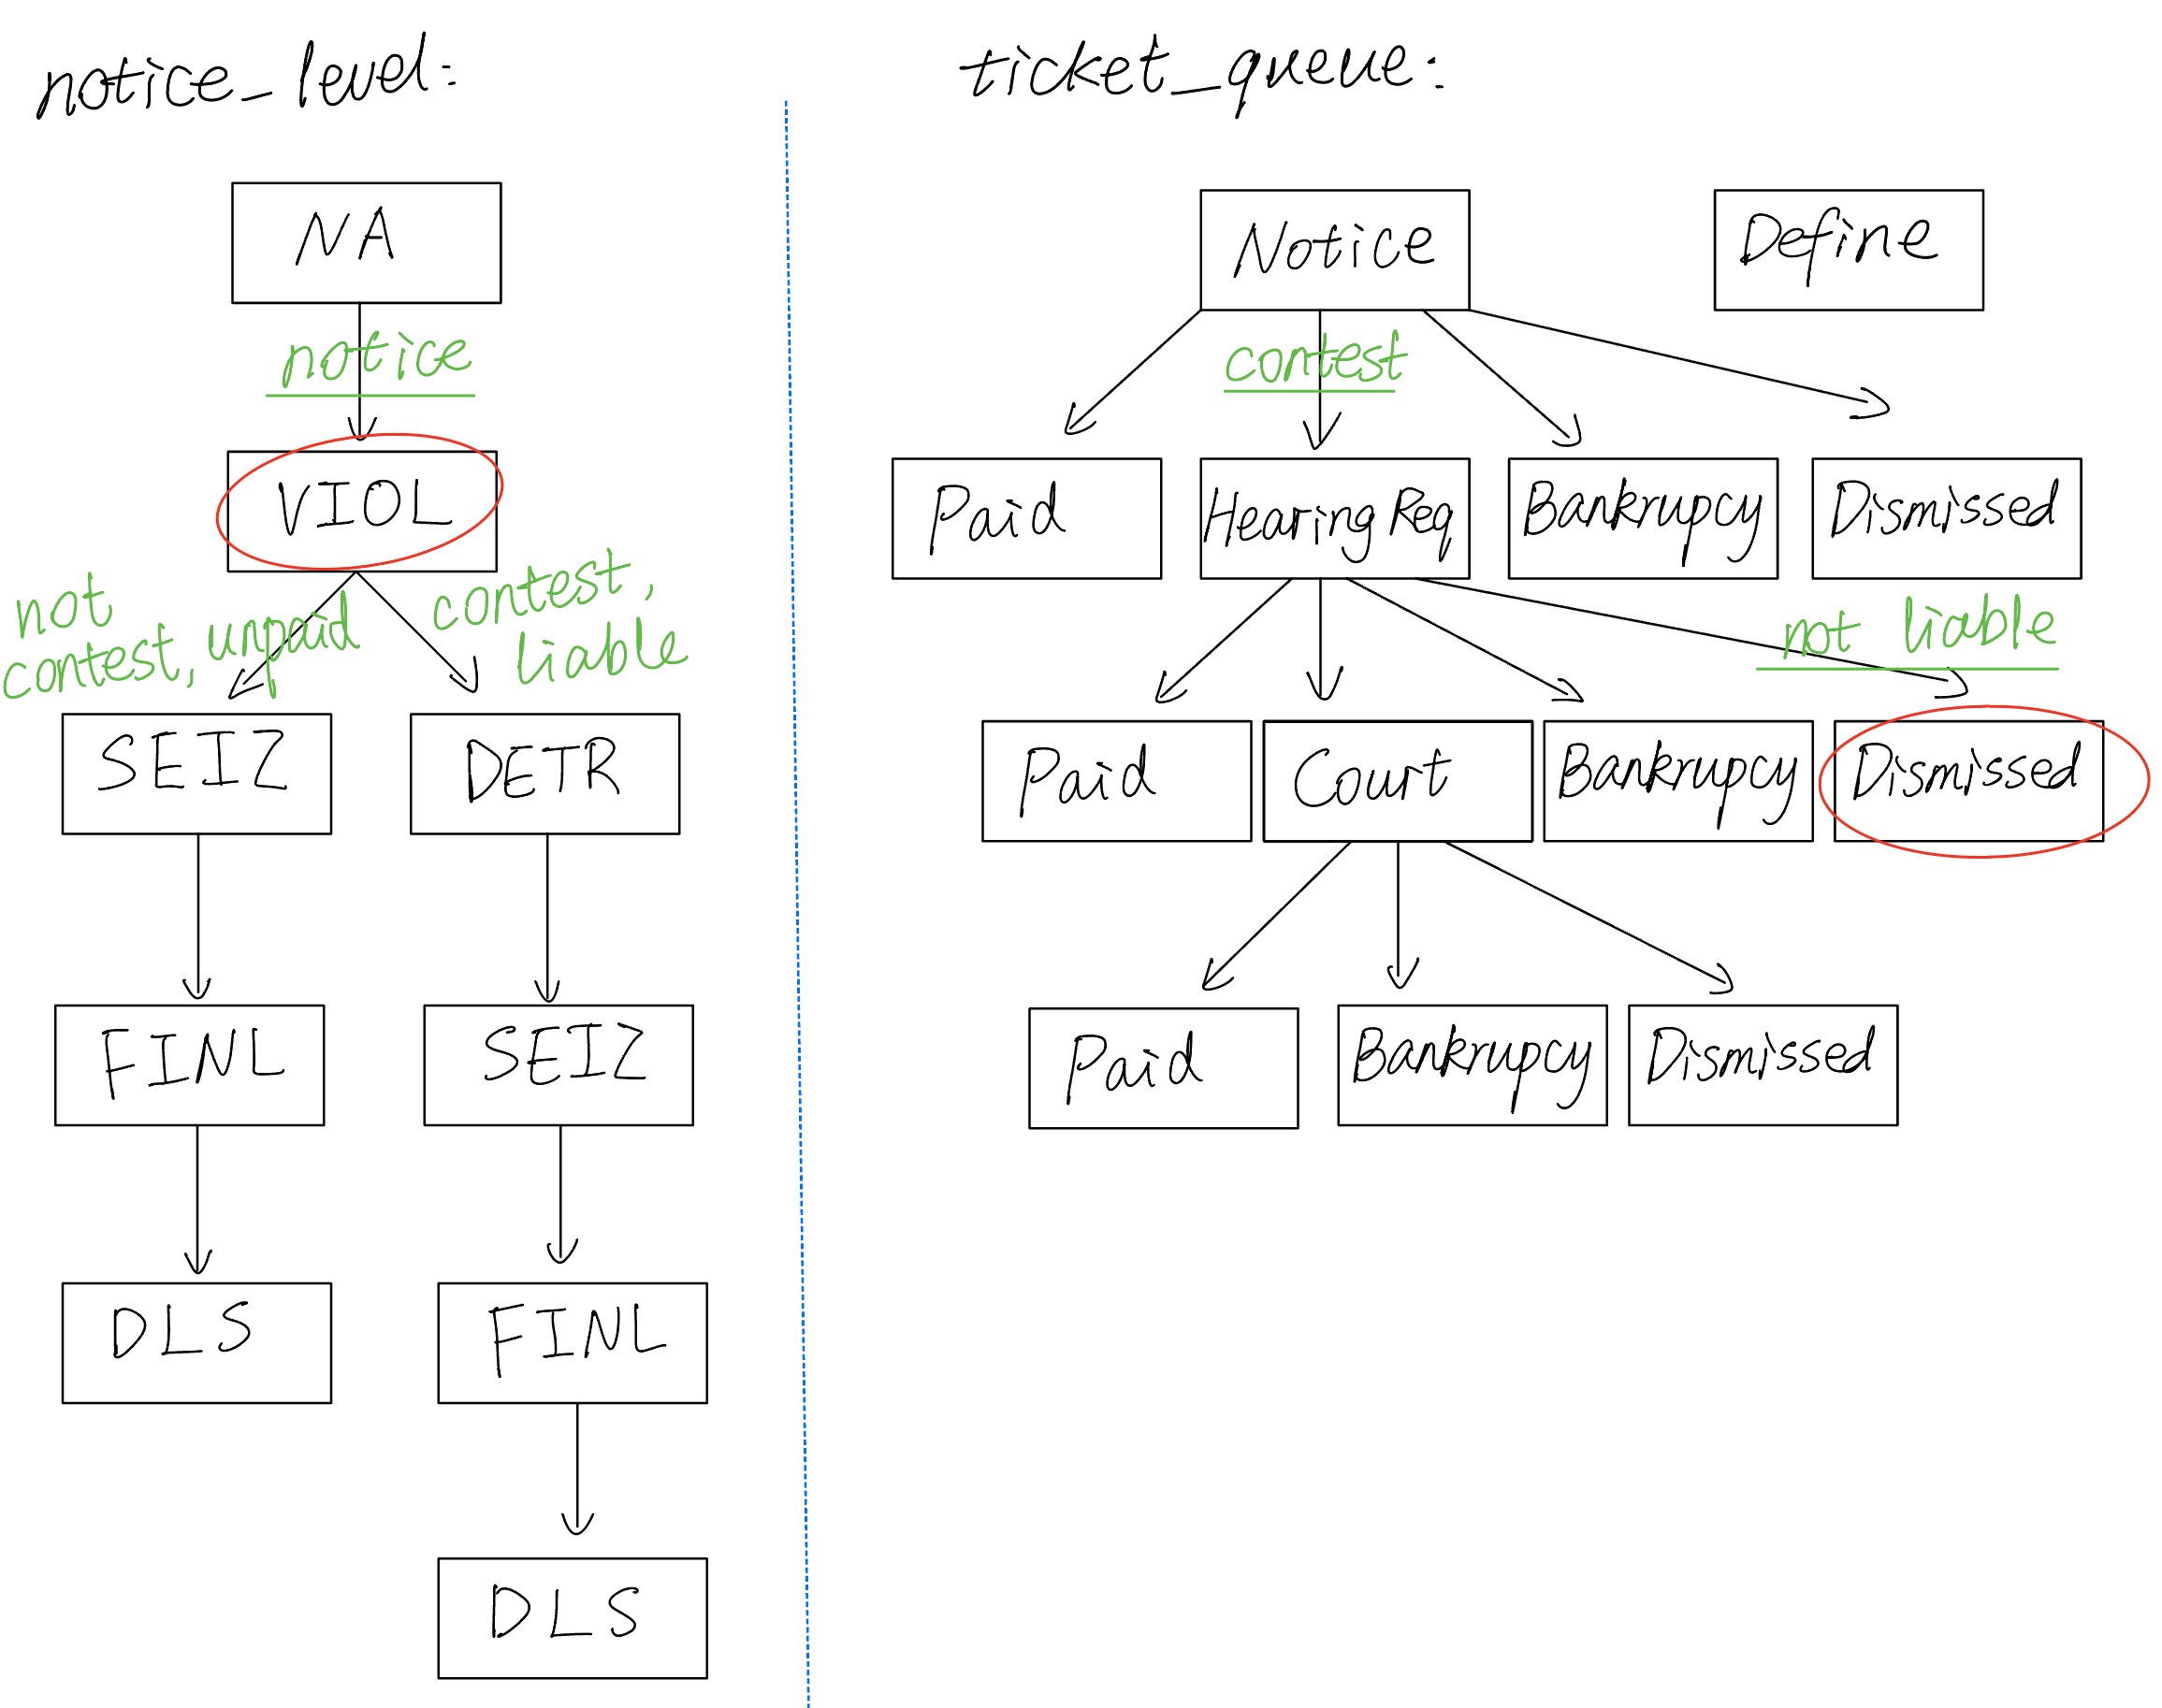
\includegraphics{./Users/hengyix/Documents/GitHub/student30538/Tree_Plot_1.jpg}




\end{document}
